% Figure 1: the two properties of the shared test files that the benchmark repairs.
% (a) day-0 anchor: the earnings release (8-K) precedes the market open for most calls,
%     so the call-date anchor puts the reaction session inside the "past" window;
% (b) company overlap: a time-ordered split keeps the same companies on both sides,
%     a company-disjoint split does not. Drawn to fit one column (~7.5 cm).
\begin{figure}[t]
\centering
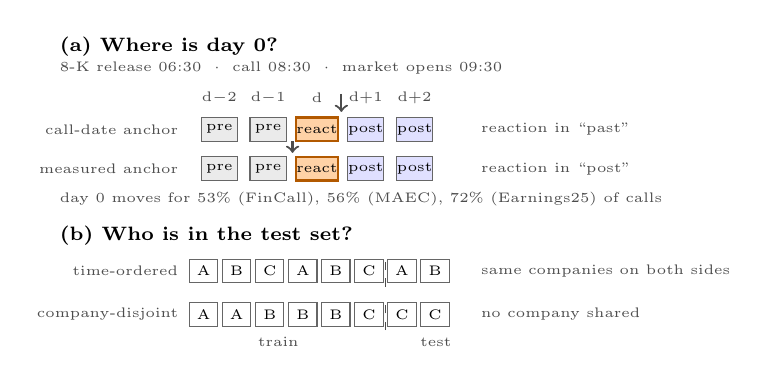
\begin{tikzpicture}[
    font=\scriptsize,
    x=1cm, y=1cm,
    sess/.style={draw=black!60, fill=white, minimum width=4.6mm, minimum height=3.0mm, inner sep=0pt, font=\tiny},
    pre/.style={sess, fill=black!8},
    post/.style={sess, fill=blue!12},
    react/.style={sess, fill=orange!35, draw=orange!70!black, thick},
    lab/.style={font=\tiny, text=black!70},
]
% ---------------------------------------------------------------- (a) anchor
\node[anchor=west, font=\scriptsize\bfseries] at (0,2.55) {(a) Where is day~0?};
\node[lab, anchor=west] at (0,2.28) {8-K release 06:30 $\;\cdot\;$ call 08:30 $\;\cdot\;$ market opens 09:30};
\foreach \i/\t in {0/d$-$2, 1/d$-$1, 2/d, 3/d$+$1, 4/d$+$2}
  \node[lab] at (2.15+\i*0.62, 1.9) {\t};
\node[lab, anchor=east] at (1.75,1.5) {call-date anchor};
\foreach \i/\s in {0/pre, 1/pre, 2/react, 3/post, 4/post}
  \node[\s] at (2.15+\i*0.62, 1.5) {\s};
\draw[->, thick, black!70] (2.15+2.5*0.62,1.95) -- (2.15+2.5*0.62,1.72);
\node[lab, anchor=west] at (5.35,1.5) {reaction in ``past''};
\node[lab, anchor=east] at (1.75,1.0) {measured anchor};
\foreach \i/\s in {0/pre, 1/pre, 2/react, 3/post, 4/post}
  \node[\s] at (2.15+\i*0.62, 1.0) {\s};
\draw[->, thick, black!70] (2.15+1.5*0.62,1.35) -- (2.15+1.5*0.62,1.2);
\node[lab, anchor=west] at (5.35,1.0) {reaction in ``post''};
\node[lab, anchor=west] at (0,0.62) {day~0 moves for 53\% (FinCall), 56\% (MAEC), 72\% (Earnings25) of calls};
% ---------------------------------------------------------------- (b) overlap
\node[anchor=west, font=\scriptsize\bfseries] at (0,0.15) {(b) Who is in the test set?};
\node[lab, anchor=east] at (1.75,-0.3) {time-ordered};
\foreach \i/\t in {0/A, 1/B, 2/C, 3/A, 4/B, 5/C, 6/A, 7/B}
  \node[sess, minimum width=3.6mm] at (1.95+\i*0.42, -0.3) {\t};
\draw[dashed, black!70] (4.26,-0.5) -- (4.26,-0.1);
\node[lab, anchor=west] at (5.35,-0.3) {same companies on both sides};
\node[lab, anchor=east] at (1.75,-0.85) {company-disjoint};
\foreach \i/\t in {0/A, 1/A, 2/B, 3/B, 4/B, 5/C, 6/C, 7/C}
  \node[sess, minimum width=3.6mm] at (1.95+\i*0.42, -0.85) {\t};
\draw[dashed, black!70] (4.26,-1.05) -- (4.26,-0.65);
\node[lab, anchor=west] at (5.35,-0.85) {no company shared};
\node[lab] at (2.9,-1.2) {train};
\node[lab] at (4.9,-1.2) {test};
\end{tikzpicture}
\caption{\textbf{Two properties of the shared test files.} (a)~Most companies
release results before the open, so anchoring day~0 on the call date places the
session in which the market reacts inside the ``past'' window; the benchmark
anchors on the measured release time. (b)~A time-ordered split keeps the same
companies on both sides, so a model can score by recognising the company; the
benchmark adds a company-disjoint split and swap checks that make the difference
measurable.}
\label{fig:problems}
\end{figure}
